\section{Methods}
\label{sec:methods}

\newcommand{\p}{\bm{p}}
\newcommand{\vv}{\bm{v}}
\newcommand{\X}{\bm{X}}
\newcommand{\Y}{\bm{Y}}
\newcommand{\M}{\bm{M}}
\newcommand{\U}{\bm{U}}
% \newcommand{\R}{\mathbb{R}}

\newcommand{\img}[2]{#1 : \Omega \to #2}
\newcommand{\binimg}[1]{\img{#1}{ \{ 0, 1 \} }}

\newcommand{\Dom}{\mathcal{D}}
\newcommand{\Tas}{\mathcal{T}}
\newcommand{\Xdo}{\mathcal{X}}
\newcommand{\Ydo}{\mathcal{Y}}
\newcommand{\fp}[1]{f_{\theta \text{#1}}}
\newcommand{\wt}{\widetilde}

% https://tex.stackexchange.com/a/466437/216202
\renewcommand*\st[1]{_{\textnormal{#1}}}

\newcommand{\post}{\st{postop}}
\newcommand{\pre}{\st{preop}}
\newcommand{\cav}{\st{cavity}}
\newcommand{\simul}{\st{sim}}
\newcommand{\lab}{\st{labeled}}
\newcommand{\unl}{\st{unlabeled}}


We describe our learning strategy in \cref{sec:learning_strategy} (\cref{fig:diagram})
and introduce our resection cavity simulation in \cref{sec:simulation}.

\begin{figure}
  \centering
  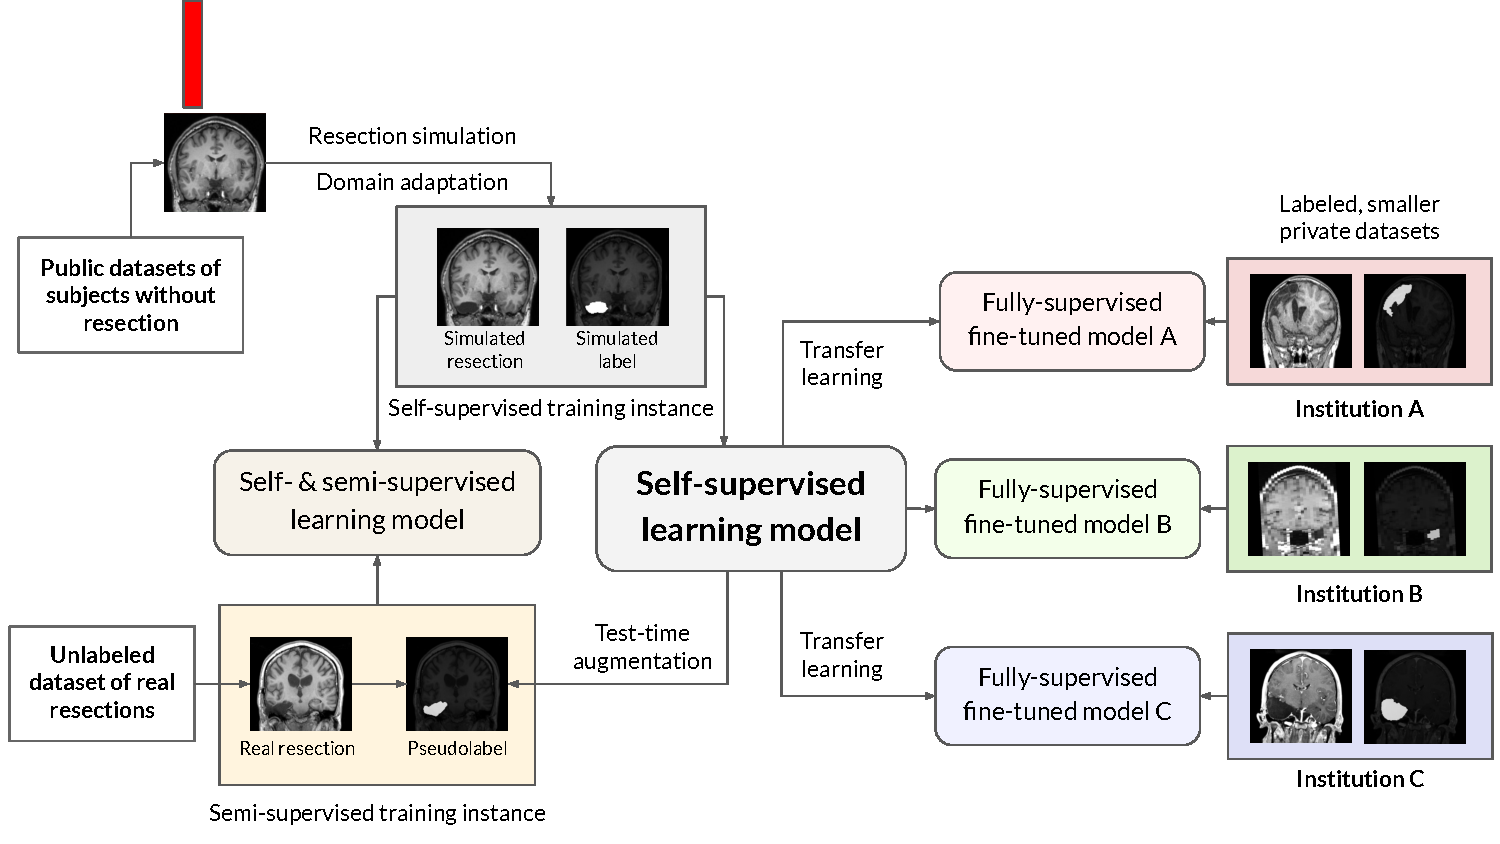
\includegraphics[trim={0 0 0 52},clip, width=\linewidth]{diagram_ijcars}
  \caption{
    Learning strategies.
    3D images without resections (top left) are modified by our resection simulation method to mimic postoperative images and their corresponding labels, generating training instances.
    These instances are used to train a baseline model in a self-supervised manner (middle).
    The baseline model generates pseudolabels from unlabeled images of patients who underwent resective surgery (bottom left).
    Instances from the resection cavity simulation and pseudolabeled dataset are used to train a new model in a self- and semi-supervised learning approach (left).
    The baseline model may be fine-tuned to improve its performance on small labeled datasets containing real resections from a single institution, using a standard fully-supervised learning approach (right).
  }
  \label{fig:diagram}
\end{figure}

\subsection{Learning strategy}
\label{sec:learning_strategy}


\subsubsection{Problem statement}

\newcommand{\loss}{\mathcal{L}}
\newcommand{\expec}{\mathbb{E}}
\newcommand{\exppost}{\expec_{\Dom\post}}

The overall objective is to automatically segment \acp{RC} from postoperative \ac{T1w} \ac{MRI} using a \ac{CNN} $f_{\bm{\theta}}$ parameterized by weights $\bm{\theta}$.
Let $\X_{\text{post}} : \Omega \to \R$ and $\Y\cav  : \Omega \to \{ 0, 1 \}$ be a postoperative \ac{T1w} \ac{MRI} and its cavity segmentation label, respectively, where $\Omega \subset \R^3$.
$\X_{\text{post}}$ and $\Y_{\text{cavity}}$ are drawn from the data distribution $\Dom\post$.
In model training, the aim is to minimize the expected discrepancy between the label $\Y\cav$ and network prediction $f_{\bm{\theta}}(\X\post)$.
Let $\loss$ be a loss function that estimates this discrepancy (e.g., Dice loss).
The optimization problem for the network parameters $\bm{\theta}$ is:
\begin{equation}
    \bm{\theta}^* =
    \argmin_{\bm{\theta}}
    \exppost \left[
        \loss \left(
            f_{\bm{\theta}} \left( \X\post \right),
            \Y\cav
        \right)
    \right]
    \label{eq:problem_optimization}
\end{equation}


In a fully-supervised setting, a labeled dataset $D\post = \{ (\X_{\text{post}_i}, \Y_{\text{cavity}_i}) \}_{i = 1}^{n\post}$ is employed to estimate the expectation defined in \cref{eq:problem_optimization} as:
\begin{equation}
    \exppost \left[
        \loss \left(
            f_{\bm{\theta}} \left( \X\post \right), \Y\cav
        \right)
    \right]
    \approx \frac{1}{n\post} \sum_{i=1}^{n\post} \loss(f_{\bm{\theta}}(\X_{\text{post}_i}), \Y_{\text{post}_i})
    \label{eq:problem_optimization_fully}
\end{equation}

In practice, \acp{CNN} typically require an annotated dataset with a large $n\post$ to generalize well for unseen instances.
However, given the time and expertise required to annotate scans, $n\post$ is often small.
We present a method to artificially increase $n\post$ by simulating postoperative \acp{MRI} and associated labels from preoperative scans.


\subsubsection{Simulation for domain adaptation and self-supervised learning}
\label{sec:sim_res_self}

Let $D\pre = \{ \X_{\text{pre}_i} \}_{i = 1}^{n\pre}$ be a dataset of preoperative \ac{T1w} \ac{MRI}, drawn from the data distribution $\Dom\pre$.
We propose to generate a simulated postoperative dataset $D\simul = \{ (\X_{\text{sim}_i}, \Y_{\text{sim}_i}) \}_{i = 1}^{n\simul}$ using the preoperative dataset $D\pre$.
Specifically, we aim to build a generative model $\phi\simul : \X\pre \mapsto (\X\simul, \Y\simul)$ that transforms preoperative images into simulated, annotated postoperative images that imitate instances drawn from the postoperative data distribution $\Dom\post$.
$D\simul$ can then be used to estimate the expectation in \cref{eq:problem_optimization}:
\begin{equation}
    \exppost \left[\
        \loss\left(
            f_{\bm{\theta}} \left(\X\post \right), \Y\cav \right)
        \right]
        \approx \frac{1}{n\simul}\sum_{i=1}^{n\simul} \loss(f_{\bm{\theta}}(\X_{\text{sim}_i}),  \Y_{\text{sim}_i})
    \label{eq:problem_optimization_sim}
\end{equation}

Simulated images can be generated from any unlabeled preoperative dataset.
Therefore, the size of the simulated dataset can be much greater than the annotated dataset $D\post$, i.e., $n\simul\gg n\post$.
The network parameters $\bm{\theta}$ can be optimized by minimizing \cref{eq:problem_optimization_sim} using stochastic gradient descent, leading to a trained predictive function $f_{\bm{\theta_}{\text{sim}}}$.
Finally, $f_{\bm{\theta_}{\text{sim}}}$ can be fine-tuned on $D\post$ to improve performance on the postoperative domain $\Dom\post$.

\subsubsection{Leveraging unlabeled data from the target domain}
\label{sec:leveraging_semi}

Let $D\unl = \{ \X_{\text{postop}_i} \}_{i = 1}^{n\st{unl}}$ be a dataset comprising $n\st{unl}$ unlabeled postoperative images.
We propose to leverage $D\unl$ to build a better predictive model than using simulated resections only, employing a semi-supervised learning approach.
First, pseudolabels for each image $\X\post \in D\unl$ can be generated with $f_{\theta_{\text{sim}}}$ using data distillation, i.e., ensembling multiple predictions from transformed versions of $\X\post$.
Using the multiple predictions generated for pseudolabels, we estimate image-level segmentation uncertainty so that only instances with high reliability are used for training.
Finally, simulated resection instances and the selected pseudolabeled instances are used to train a new model $f_{\theta_{\text{sim+unl}}}$ in a hybrid self- and semi-supervised setting.


\paragraph{Generating pseudolabels using data distillation}

Data distillation is a method that ensembles predictions from multiple transformations applied to data, using a single model \cite{radosavovic_data_2017}.
We use Monte Carlo simulation to generate each pseudolabel with \ac{TTA}, which can improve the performance of segmentation models \cite{wang_aleatoric_2019}.
Let $n\st{u}$ represent the total number of simulation runs.
In the $i$-th simulation run,
the \ac{TTA} intensity and spatial transforms $T_\alpha$ and $T_\beta$ (\cref{sec:preprocessing_augmentation}) are applied to $\X\post$.
$\fp{sim}$ is used to predict $\wt{\Y}_{\theta\alpha\beta}'$, the probability of each voxel belonging to the cavity in the transformed space.
Finally, $T_\beta^{-1}$ is used to transform $\wt{\Y}_{\theta\alpha\beta}'$ back onto the space of $\X\post$:
\begin{equation}
    \wt{\Y}'_{\text{cavity}_i}
    = T_\beta^{-1}
    \circ \fp{sim}
    \circ T_\beta
    \circ T_\alpha
    \circ \X\post
    = T_\beta^{-1} \left( \wt{\Y}_{\theta\alpha\beta}' \right)
\end{equation}

We ensure that $T_\beta$ is invertible by using diffeomorphic spatial transformations.
To preserve image quality and ensure that probabilities stay within $[0, 1]$, we use tricubic and trilinear interpolation for $T_\beta$ and $T_\beta^{-1}$, respectively.

Predictions $P = \{ \wt{\Y}'_{\text{cavity}_i} \}_{i=1}^{n\st{u}}$ are averaged to obtain $\img{\wt{\Y}\cav}{[0, 1]}$, and the corresponding binary pseudolabel $\binimg{\widetilde{\Y}\cav}$ is obtained applying a threshold of 0.5 to $\wt{\Y}'\cav$.


\paragraph{Uncertainty estimation as selection criterion for pseudolabeled instances}

Images in $D\unl$ might have artifacts that limit the quality of the segmentation or include \acp{rc} not modeled by $\phi\simul$.
The corresponding noisy pseudolabels would hinder training of machine learning models.

As $n\st{unl}$ might be large, rather than performing manual quality control to select pseudolabels with high reliability for training, we use uncertainty estimation as an automated selection criterion \cite{venturini_uncertainty_2020}.

We use $n\st{unc}$ \ac{TTA} predictions to estimate aleatoric uncertainty, which captures noise inherent in the observation \cite{kendall_what_2017}.
Aleatoric uncertainty can indicate segmentation quality and is a successful selection criterion of pseudolabels in semi-supervised learning settings for medical image segmentation \cite{wang_aleatoric_2019,venturini_uncertainty_2020}.

Let $L = \{ l_i \}_{i = 1}^{n\st{unc}}$ denote the set of (soft) volumes of the segmented cavity for each prediction, where $l_i$ is the sum of all probabilities in the $i$-th prediction $\wt{\Y}'_{\text{cavity}_i} \in P$.
We use the \ac{CQV} of the volumes \cite{zwillinger_crc_1999,wang_aleatoric_2019} to estimate the image-level uncertainty $u : L \to \left[0, 1\right]$:
\begin{equation}
    u = \frac{q_3 - q_1}{q_3 + q_1}
\end{equation}
where $q_1$ and $q_3$ are the first and third quartiles of $L$, respectively.
The \ac{CQV} is agnostic to the volume of the segmented \ac{rc} and therefore avoids bias introduced by naturally-occurring uncertainty along the resection boundaries \cite{jungo_analyzing_2020}.
Finally, training instances with an associated prediction uncertainty $u(f_{\theta\alpha\beta}, \X\post, n\st{unc})$ below a threshold $t\st{unc}$ are combined with self-labeled instances (\cref{sec:sim_res_self}) to train a new model.

\subsection{Resection simulation for self-supervised learning}
\label{sec:simulation}

\newcommand{\AAA}{\bm{A}}
\newcommand{\NN}{\mathcal{N}}


$\phi\simul$ takes images from $\Dom\pre$ to generate training instances by simulating a realistic shape, location and intensity pattern for the \ac{RC}.
We present simulation of cavity shape and label in \cref{sec:cavity,sec:cavity_constrain}, respectively.
In \cref{sec:texture_cavity}, we present our method to generate the resected image.


\subsubsection{Initial cavity shape}
\label{sec:cavity}

To simulate a realistic \ac{RC}, we consider its topological and geometric properties: it is a single volume with a non-smooth boundary.
We generate a geodesic polyhedron with frequency $f$ by subdividing the edges of an icosahedron $f$ times and projecting each vertex onto a parametric sphere with a unit radius centered at the origin.
This polyhedron models a spherical surface $S = \{ V, F \}$ with vertices
$
  V = \left\{
    \vv_i \in \R^3
  \right\}
  _{i = 1}^{n_V}
$
and faces
$
  F = \left\{
    \bm{f}_k \in \mathbb{N}^3
  \right\}
  _{k = 1}^{n_F}
$, where $n_V$ and $n_F$ are the number of vertices and faces, respectively.
%
Each face $\bm{f}_k = \{ i_1^k, i_2^k, i_3^k \}$ is a sequence of three non-repeated vertex indices.

To create a non-smooth surface, $S$ is perturbed with simplex noise \cite{perlin_improving_2002}, a procedural noise generated by interpolating pseudorandom gradients on a multidimensional simplicial grid.
We chose simplex noise as it simulates natural-looking textures or terrains and is computationally efficient for multiple dimensions.
The noise $\eta : \R^3 \to [-1, 1]$ at point $\p \in \R^3$ is a weighted sum of the noise contribution for $\omega$ different octaves, with weights $\{\gamma ^ {n - 1}\}_{n = 1}^{\omega}$ controlled by the persistence parameter $\gamma$.
The displacement $\delta$ of a vertex $\vv$ is:
\begin{equation}
  \delta(\vv)
  = \eta \left( \frac{\vv + \bm{\mu} }{\zeta}, \omega, \gamma \right)
\end{equation}
where
$\zeta$ is a scaling parameter to control smoothness
and $\bm{\mu}$ is a shifting parameter that adds stochasticity
(equivalent to a random number generator seed).
%
Each vertex $\vv_i$ is displaced radially to create a perturbed sphere:
$
V_{\delta}
  = \left\{
  \vv_i
  + \delta(\vv_i)
  \frac{\vv_i}{\|\vv_i\|}
  \right\}
  _{i = 1}^{n_V}
  = \left\{
  \vv_{\delta i}
  \right\}
  _{i = 1}^{n_V}
$.

Next, a series of transforms is applied to $V_{\delta}$ to modify the mesh's volume and shape.
To add stochasticity, random rotations around each axis are applied to $V_{\delta}$ with the rotation transform
$T\st{R}(\bm{\theta}\st{r}) = R_x(\theta_x) \circ R_y(\theta_y) \circ R_z(\theta_z)$,
where~$\circ$~indicates a transform composition and
$R_i(\theta_i)$ is a rotation of $\theta_i$ radians around axis $i$.
$T\st{S}(\bm{r})$ is a scaling transform,
where $(r_1, r_2, r_3) = \bm{r}$ are semiaxes of an ellipsoid
with volume $v$ used to model the cavity shape.
The semiaxes are computed as
$r_1 = r$, $r_2 = \lambda r$ and $r_3 = r /\lambda$,
where $r = (3 v / 4)^{1/3}$ and
$\lambda$ controls the semiaxes length ratios\footnote{
  Note the volume of an ellipsoid with semiaxes $(a, b, c)$ is $v = \frac{4}{3} \pi a b c$.
}.
These transforms are applied to $V_{\delta}$ to define the initial \ac{RC} surface $S\st{E} = \{ V\st{E}, F \}$, where
$V\st{E} =
\{
  T\st{S}(\bm{r})
  \circ T\st{R}(\bm{\theta}\st{r})(
    \vv_{\delta i})
\}
_{i = 1}^{n_V}
$.


\subsubsection{Cavity label}
\label{sec:cavity_constrain}


\begin{figure}
  \centering
  % \captionsetup[subfigure]{justification=centering}
  \begin{subfigure}{0.3\textwidth}
    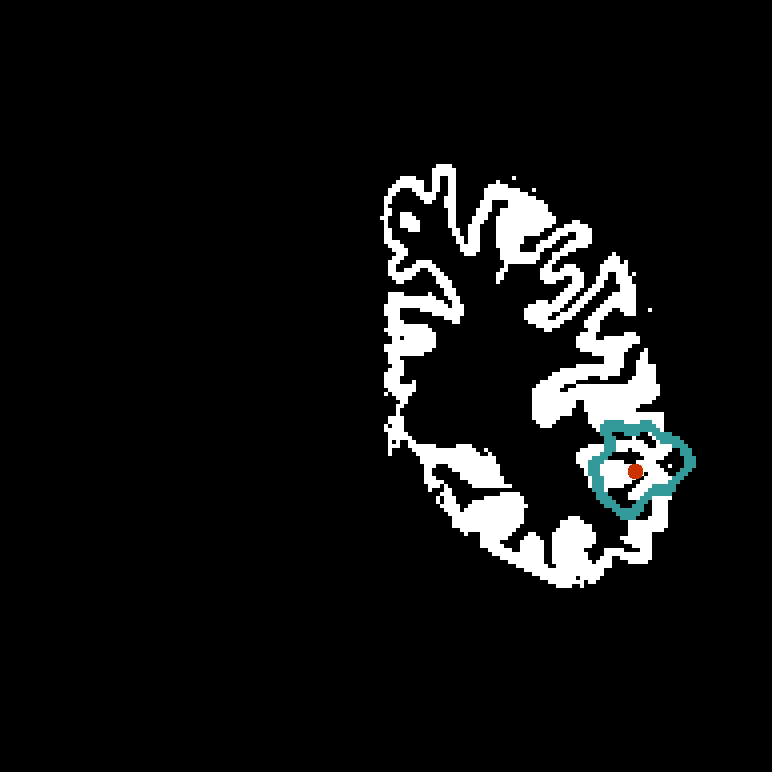
\includegraphics[width=0.8\linewidth]{Ma}
    \caption{$S_a$ on $\M\st{GM}^h$\label{fig:sama}}
  \end{subfigure}
  \begin{subfigure}{0.3\textwidth}
    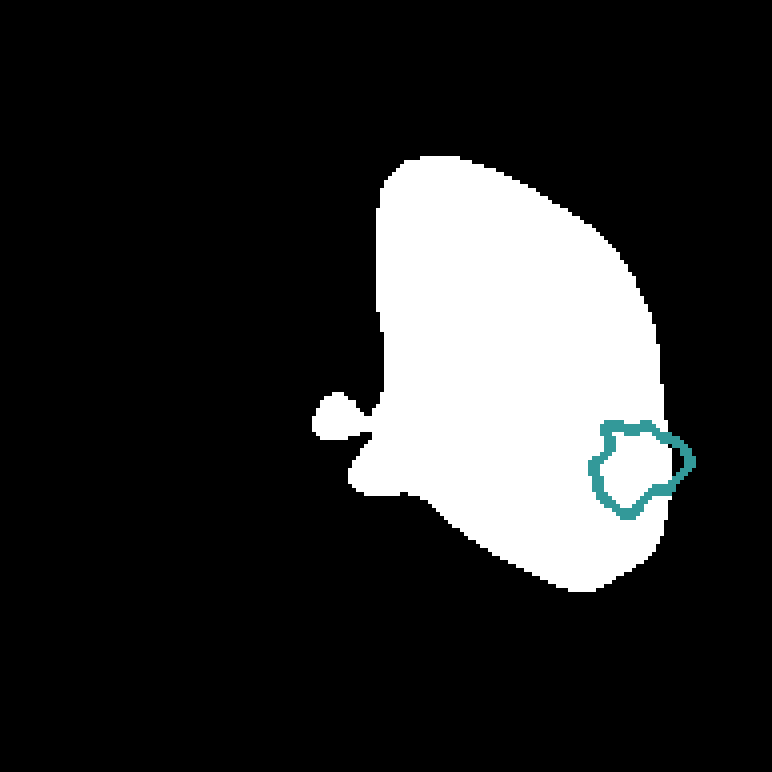
\includegraphics[width=0.8\linewidth]{Mb}
    \caption{$S_a$ on $\M\st{R}^h$\label{fig:samb}}
  \end{subfigure}
  \begin{subfigure}{0.3\textwidth}
    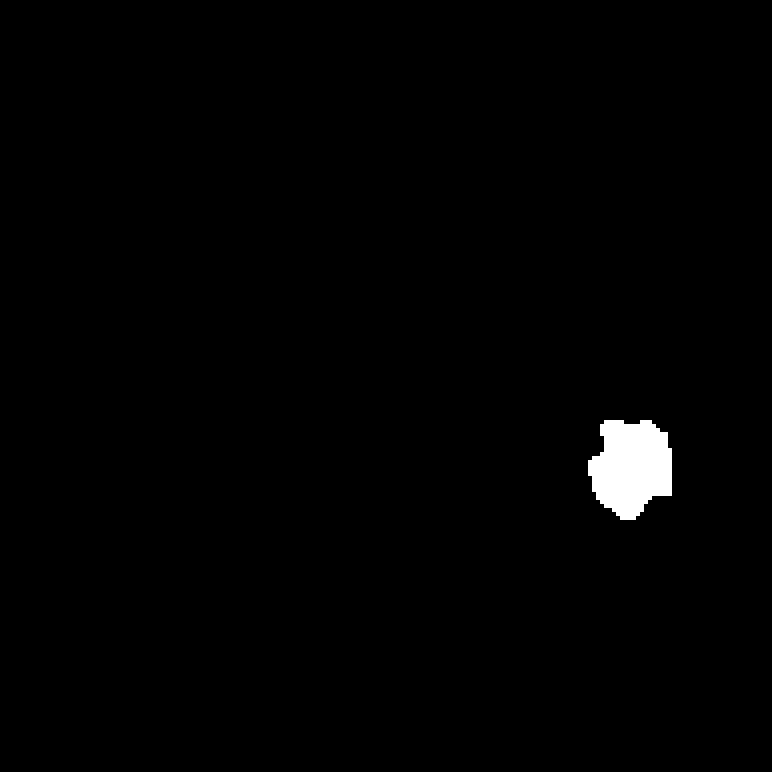
\includegraphics[width=0.8\linewidth]{Mr}
    \caption{$\Y\simul = \M_{S_a} \odot \M\st{R}^h$\label{fig:mr}}
  \end{subfigure}

  \caption[Simulation of the ground-truth cavity label]{
    Simulation of the ground-truth cavity label.
    $S_a$ (blue) is computed by centering $S\st{E}$ on $\bm{a}$, a random positive voxel (red) of $\M\st{GM}^h$ (\subref{fig:sama}).
    $\M_{S_a}$ is a binary mask derived from $S_a$.
    $\Y\simul$ (\subref{fig:mr}) is the intersection of $\M_{S_a}$ and $\M\st{R}^h$ (\subref{fig:samb}).
  }
  \label{fig:shape}
\end{figure}



The simulated \ac{RC} should not span both hemispheres or include extracerebral tissues such as bone or scalp.
This section describes our method to ensure that the \ac{RC} appears in anatomically plausible regions.

A \ac{T1w} \ac{MRI} is defined as $\X\pre : \Omega \to \R$.
A full brain parcellation $\bm{P} : \Omega \to Z$ is generated \cite{cardoso_geodesic_2015} for $\X\pre$,
where $Z$ is the set of segmented structures.
A cortical gray matter mask $\M\st{GM}^h : \Omega \to \{0, 1\}$
of hemisphere $h$ is extracted from $\bm{P}$,
where $h$ is randomly chosen from $H = \{\text{left}, \text{right}\}$ with equal probability.

A ``resectable hemisphere mask'' $\M\st{R}^h$ is generated from $\bm{P}$ and $h$ such that $\M\st{R}^h (\p) = 1$ if
${\bm{P}(\p) \neq \{M\st{BG}, M\st{BT}, M\st{CB}, M_{\hat{h}} \} }$
and $0$ otherwise,
where $M\st{BG}$, $M\st{BT}$, $M\st{CB}$ and $M_{\hat{h}}$ are the labels in $Z$ corresponding to the background, brainstem, cerebellum and contralateral hemisphere, respectively.
$\M\st{R}^h$ is smoothed using a series of binary morphological operations, for realism.


A random voxel $\bm{a} \in \Omega$ is selected such that $\M\st{GM}^h(\bm{a}) = 1$.
A translation transform $T\st{T}(\bm{a} - \bm{c})$ is applied to $S\st{E}$ so $S_a = T\st{T}(\bm{a} - \bm{c}) (S\st{E})$ is centered on $\bm{a}$.

A binary image $\binimg{\M_{S_a}}$ is generated from $S_a$ such that $\M_{S_a}(\p) = 1$ for all $\p$ within $S_a$ and $\M_{S_a}(\p) = 0$ outside.
Finally, $\M_{S_a}$ is restricted by $\M\st{R}^h$ to generate the cavity label $\Y\simul = \M_{S_a} \odot \M\st{R}^h$, where $\odot$ represents the Hadamard product.
\cref{fig:shape} illustrates the process.



\subsubsection{Simulating cavities filled with CSF}
\label{sec:texture_cavity}

Brain \acp{RC} are typically filled with \ac{CSF}.
To generate a realistic \acs{CSF} texture,
we create a ventricle mask
${\M\st{V} : \Omega \to \{ 0, 1 \}}$ from $\bm{P}$, such that
$\M\st{V}(\p) = 1$ for all $\p$ within the ventricles and
$\M\st{V}(\p) = 0$ outside.
Intensity values within the ventricles are assumed to have
a normal distribution \cite{gudbjartsson_rician_1995}
with a mean $\mu\st{CSF}$ and standard deviation $\sigma\st{CSF}$
calculated from voxel intensity values in
$\{ \X\pre(\p) \mid \p \in \Omega \land \M\st{V}(\p) = 1 \}$.
A \acs{CSF}-like image is then generated as $\X\st{CSF}(\p) \sim \NN (\mu\st{CSF}, \sigma\st{CSF}), \forall \p \in \Omega$.


We use $\Y\simul$ to guide blending of $\X\st{CSF}$ and $\X\pre$ as follows.
A Gaussian filter is applied to $\Y\simul$ to obtain a smooth alpha channel $\img{\AAA_\alpha}{[0, 1]}$ defined as
$
  \AAA_\alpha
  = \Y\simul
  * \bm{G}_{\NN}(\bm{\sigma}),
$
where
$*$ is the convolution operator
and $\bm{G}_{\NN}(\bm{\sigma})$ is a 3D Gaussian kernel with standard deviations
$\bm{\sigma} = (\sigma_x, \sigma_y, \sigma_z)$.
Then, $\X\st{CSF}$ and $\X\pre$ are blended by the convex combination
\begin{equation}
  \X\simul
  = \AAA_\alpha \odot \X\st{CSF}
  + (1 - \AAA_\alpha) \odot \X\pre
\end{equation}

We use $\bm{\sigma} > 0$ to mimic partial-volume effects at the cavity boundary.
The blending process is illustrated in \cref{fig:texture}.


\begin{figure}
  \centering
  \captionsetup[subfigure]{aboveskip=3pt, belowskip=5pt}

  \begin{subfigure}{0.15\textwidth}
    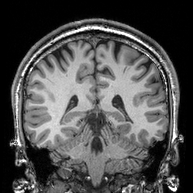
\includegraphics[width=0.99\linewidth]{texture_mri}
    \caption{\label{fig:tmri}}
  \end{subfigure}
  \begin{subfigure}{0.15\textwidth}
    
\includegraphics[width=0.99\linewidth]{texture_checkerboard}
    \caption{\label{fig:checkerboard}}
  \end{subfigure}
  \begin{subfigure}{0.15\textwidth}
    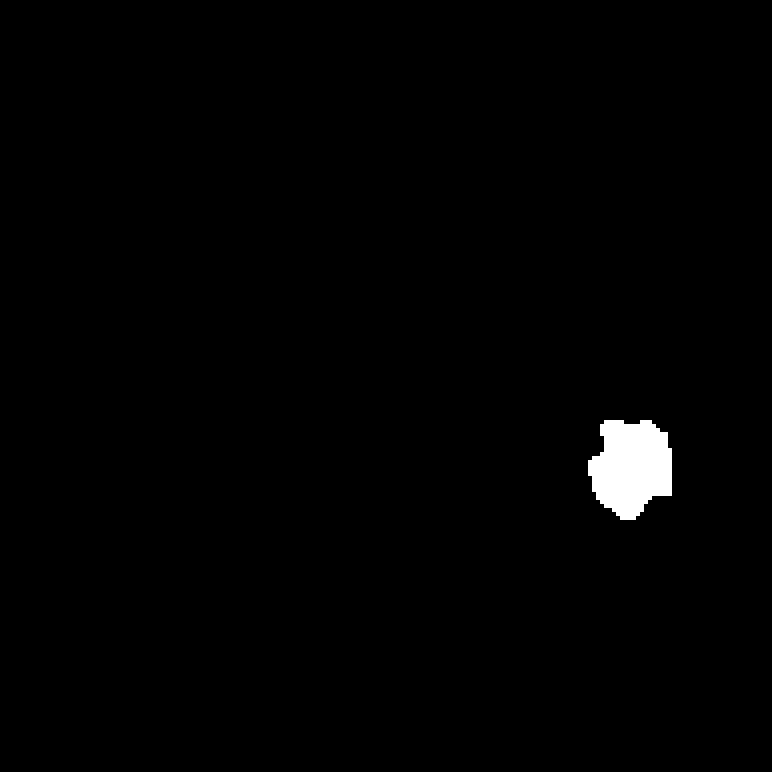
\includegraphics[width=0.99\linewidth]{Mr}
    \caption{\label{fig:tmh}}
  \end{subfigure}
  \begin{subfigure}{0.15\textwidth}
    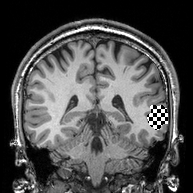
\includegraphics[width=0.99\linewidth]{texture_hard}
    \caption{\label{fig:blh}}
  \end{subfigure}
  \begin{subfigure}{0.15\textwidth}
    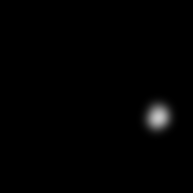
\includegraphics[width=0.99\linewidth]{texture_mask_soft}
    \caption{\label{fig:tms}}
  \end{subfigure}
  \begin{subfigure}{0.15\textwidth}
    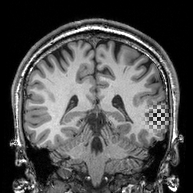
\includegraphics[width=0.99\linewidth]{texture_soft}
    \caption{\label{fig:bls}}
  \end{subfigure}

  \caption[Simulation of resected image using alpha blending]{
    Simulation of resected image $\X\simul$.
    We use a checkerboard for visualization.
    Two scalar-valued images $\X\pre$ (\subref{fig:tmri})
    and $\X_2$ (\subref{fig:checkerboard})
    are blended using $\Y\simul$ (\subref{fig:tmh})
    and $\sigma_i = \SI{0}{\milli \meter}$ to create an image with hard boundaries (\subref{fig:blh})
    and $\sigma_i = \SI{5}{\milli \meter}$ (\subref{fig:tms})
    for an image with soft boundaries (\subref{fig:bls}),
    mimicking partial-volume effects.
  }
  \label{fig:texture}
\end{figure}

